\documentclass[11pt,a4paper]{article}
\usepackage[utf8]{inputenc}
\usepackage[T1]{fontenc}
\usepackage{amsmath,amsfonts,amssymb}
\usepackage{graphicx}
\usepackage[margin=1in]{geometry}
\usepackage{listings}
\usepackage{xcolor}
\usepackage{hyperref}
\usepackage{booktabs}
\usepackage{array}
\usepackage{longtable}
\usepackage{float}
\usepackage{enumitem}

% Configure listings for Java code
\lstdefinestyle{javastyle}{
    language=Java,
    backgroundcolor=\color{gray!10},
    basicstyle=\footnotesize\ttfamily,
    keywordstyle=\color{blue}\bfseries,
    commentstyle=\color{green!60!black},
    stringstyle=\color{red},
    numberstyle=\tiny\color{gray},
    stepnumber=1,
    numbersep=5pt,
    frame=single,
    rulecolor=\color{black!30},
    breaklines=true,
    showstringspaces=false,
    tabsize=2
}

% Configure listings for bash
\lstdefinestyle{bashstyle}{
    language=bash,
    backgroundcolor=\color{gray!5},
    basicstyle=\footnotesize\ttfamily,
    keywordstyle=\color{blue}\bfseries,
    commentstyle=\color{green!60!black},
    frame=single,
    rulecolor=\color{black!30},
    breaklines=true,
    showstringspaces=false
}

\lstset{style=javastyle}

\title{Extended Testing Regime for rmatch:\\Comprehensive Performance Validation and Optimization Guidance}
\author{Performance Engineering Proposal}
\date{\today}

\begin{document}

\maketitle

\begin{abstract}
This proposal outlines an extended testing regime for the rmatch regular expression matching library to provide more challenging and diverse test scenarios that enable better assessment of performance improvements and optimization efforts. The current benchmark tests are insufficient for evaluating complex performance characteristics and guiding optimization decisions. We propose a comprehensive suite of test scenarios, metrics, and evaluation frameworks that will provide clearer insights into performance bottlenecks and optimization opportunities.
\end{abstract}

\tableofcontents
\newpage

\section{Executive Summary}

The rmatch library currently lacks comprehensive testing scenarios that can effectively guide performance optimization efforts. The existing benchmarks, while functional, do not provide sufficient diversity in test cases to reveal performance characteristics across different usage patterns, pattern complexities, and input characteristics.

This proposal presents:
\begin{itemize}
    \item A comprehensive taxonomy of test scenarios covering diverse regex patterns and input characteristics
    \item Advanced performance metrics beyond simple throughput measurements
    \item Automated test generation and validation frameworks
    \item Integration with existing CI/CD pipelines for continuous performance monitoring
    \item Clear guidance for interpreting results and prioritizing optimization efforts
\end{itemize}

\section{Problem Analysis}

\subsection{Current Testing Limitations}

The existing benchmark infrastructure has several limitations that hinder effective performance optimization:

\begin{enumerate}
    \item \textbf{Limited Pattern Diversity}: Current tests focus primarily on simple word-matching patterns from literary text
    \item \textbf{Insufficient Input Variety}: Testing is concentrated on a single corpus (Wuthering Heights)
    \item \textbf{Basic Metrics}: Performance evaluation relies mainly on throughput and memory usage
    \item \textbf{No Stress Testing}: Lack of tests for edge cases, pathological patterns, or extreme scale scenarios
    \item \textbf{Missing Regression Detection}: No systematic approach to detect performance regressions across different optimization approaches
\end{enumerate}

\subsection{Impact on Optimization Efforts}

These limitations create several challenges for performance optimization:

\begin{itemize}
    \item Difficulty in identifying which optimizations provide real-world benefits
    \item Risk of optimizing for narrow use cases while degrading performance elsewhere
    \item Inability to validate optimization effectiveness across diverse scenarios
    \item Lack of confidence in performance improvements due to limited test coverage
\end{itemize}

\section{Proposed Testing Framework}

\subsection{Test Categories}

We propose organizing tests into several categories that cover different aspects of performance:

\subsubsection{Pattern Complexity Tests}

\begin{figure}[H]
\centering
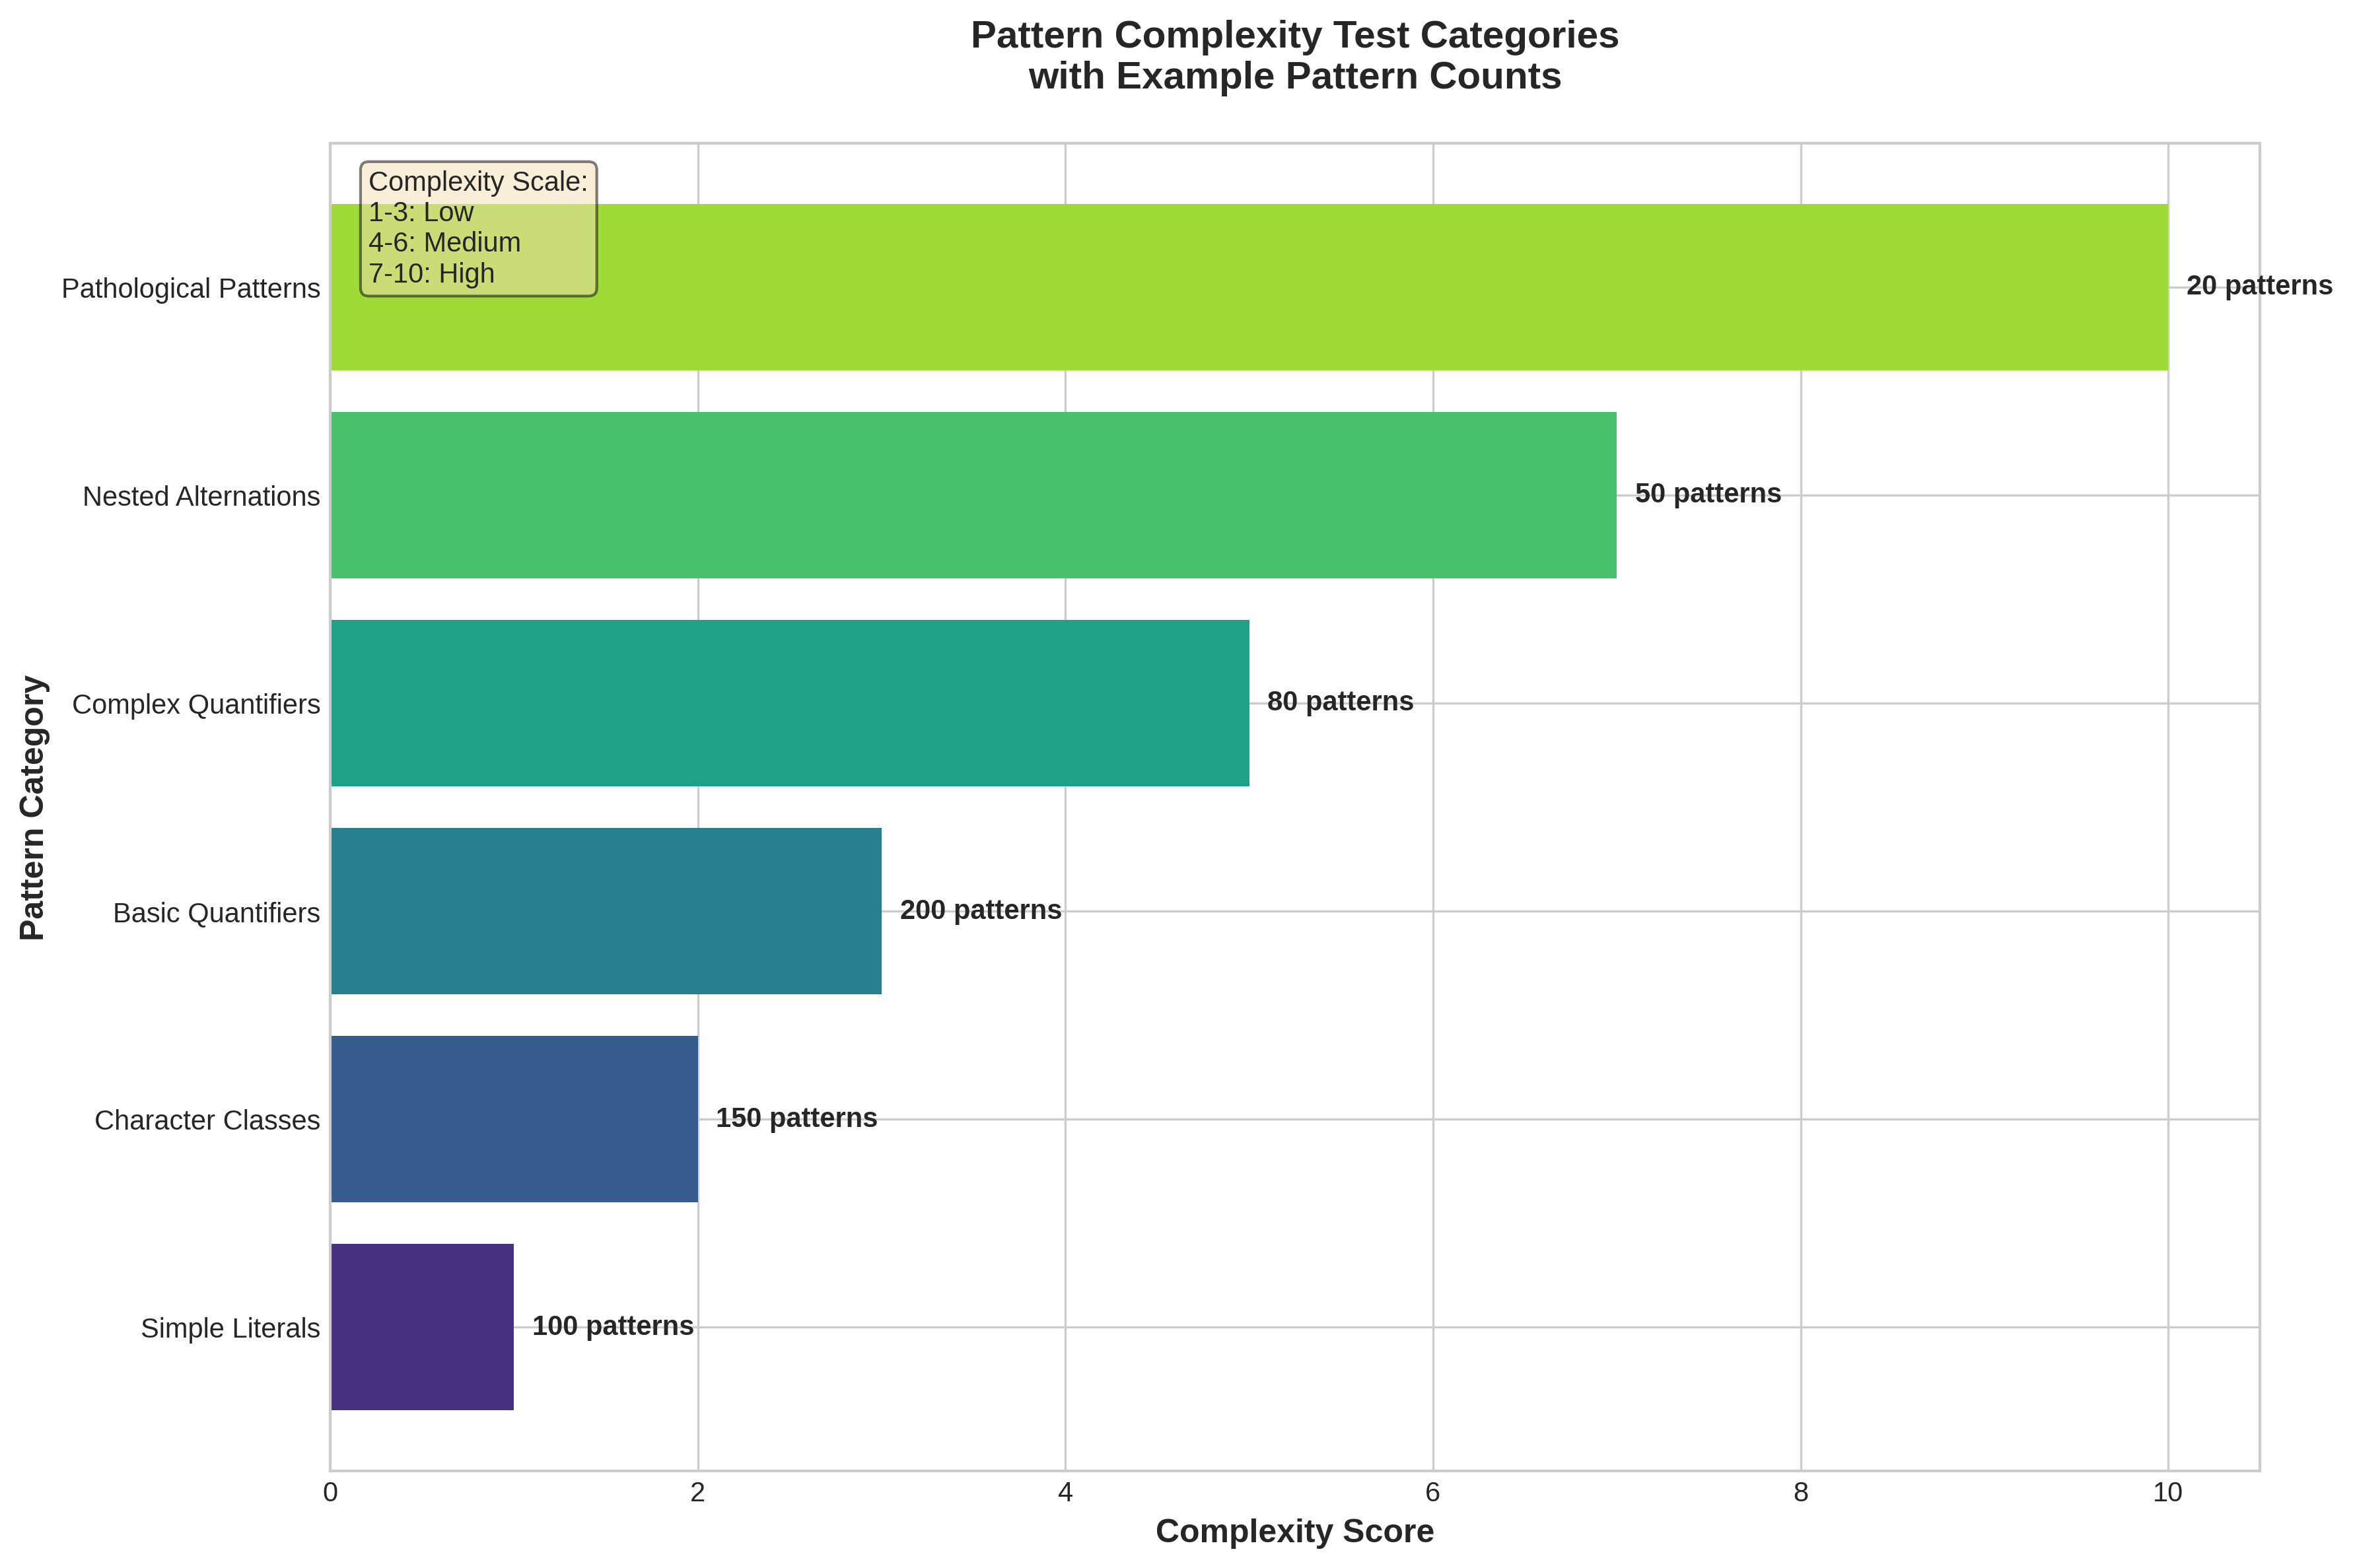
\includegraphics[width=0.8\textwidth]{illustrations/pattern_complexity_taxonomy.png}
\caption{Pattern Complexity Test Categories}
\label{fig:pattern_complexity}
\end{figure}

\begin{enumerate}
    \item \textbf{Simple Literal Patterns}: Basic string matching scenarios
    \item \textbf{Character Class Patterns}: Testing various character class implementations
    \item \textbf{Quantifier Stress Tests}: Patterns with complex quantifier combinations
    \item \textbf{Alternation Complexity}: Nested and complex alternation patterns
    \item \textbf{Pathological Patterns}: Known problematic patterns for regex engines
\end{enumerate}

\subsubsection{Input Characteristic Tests}

\begin{figure}[H]
\centering
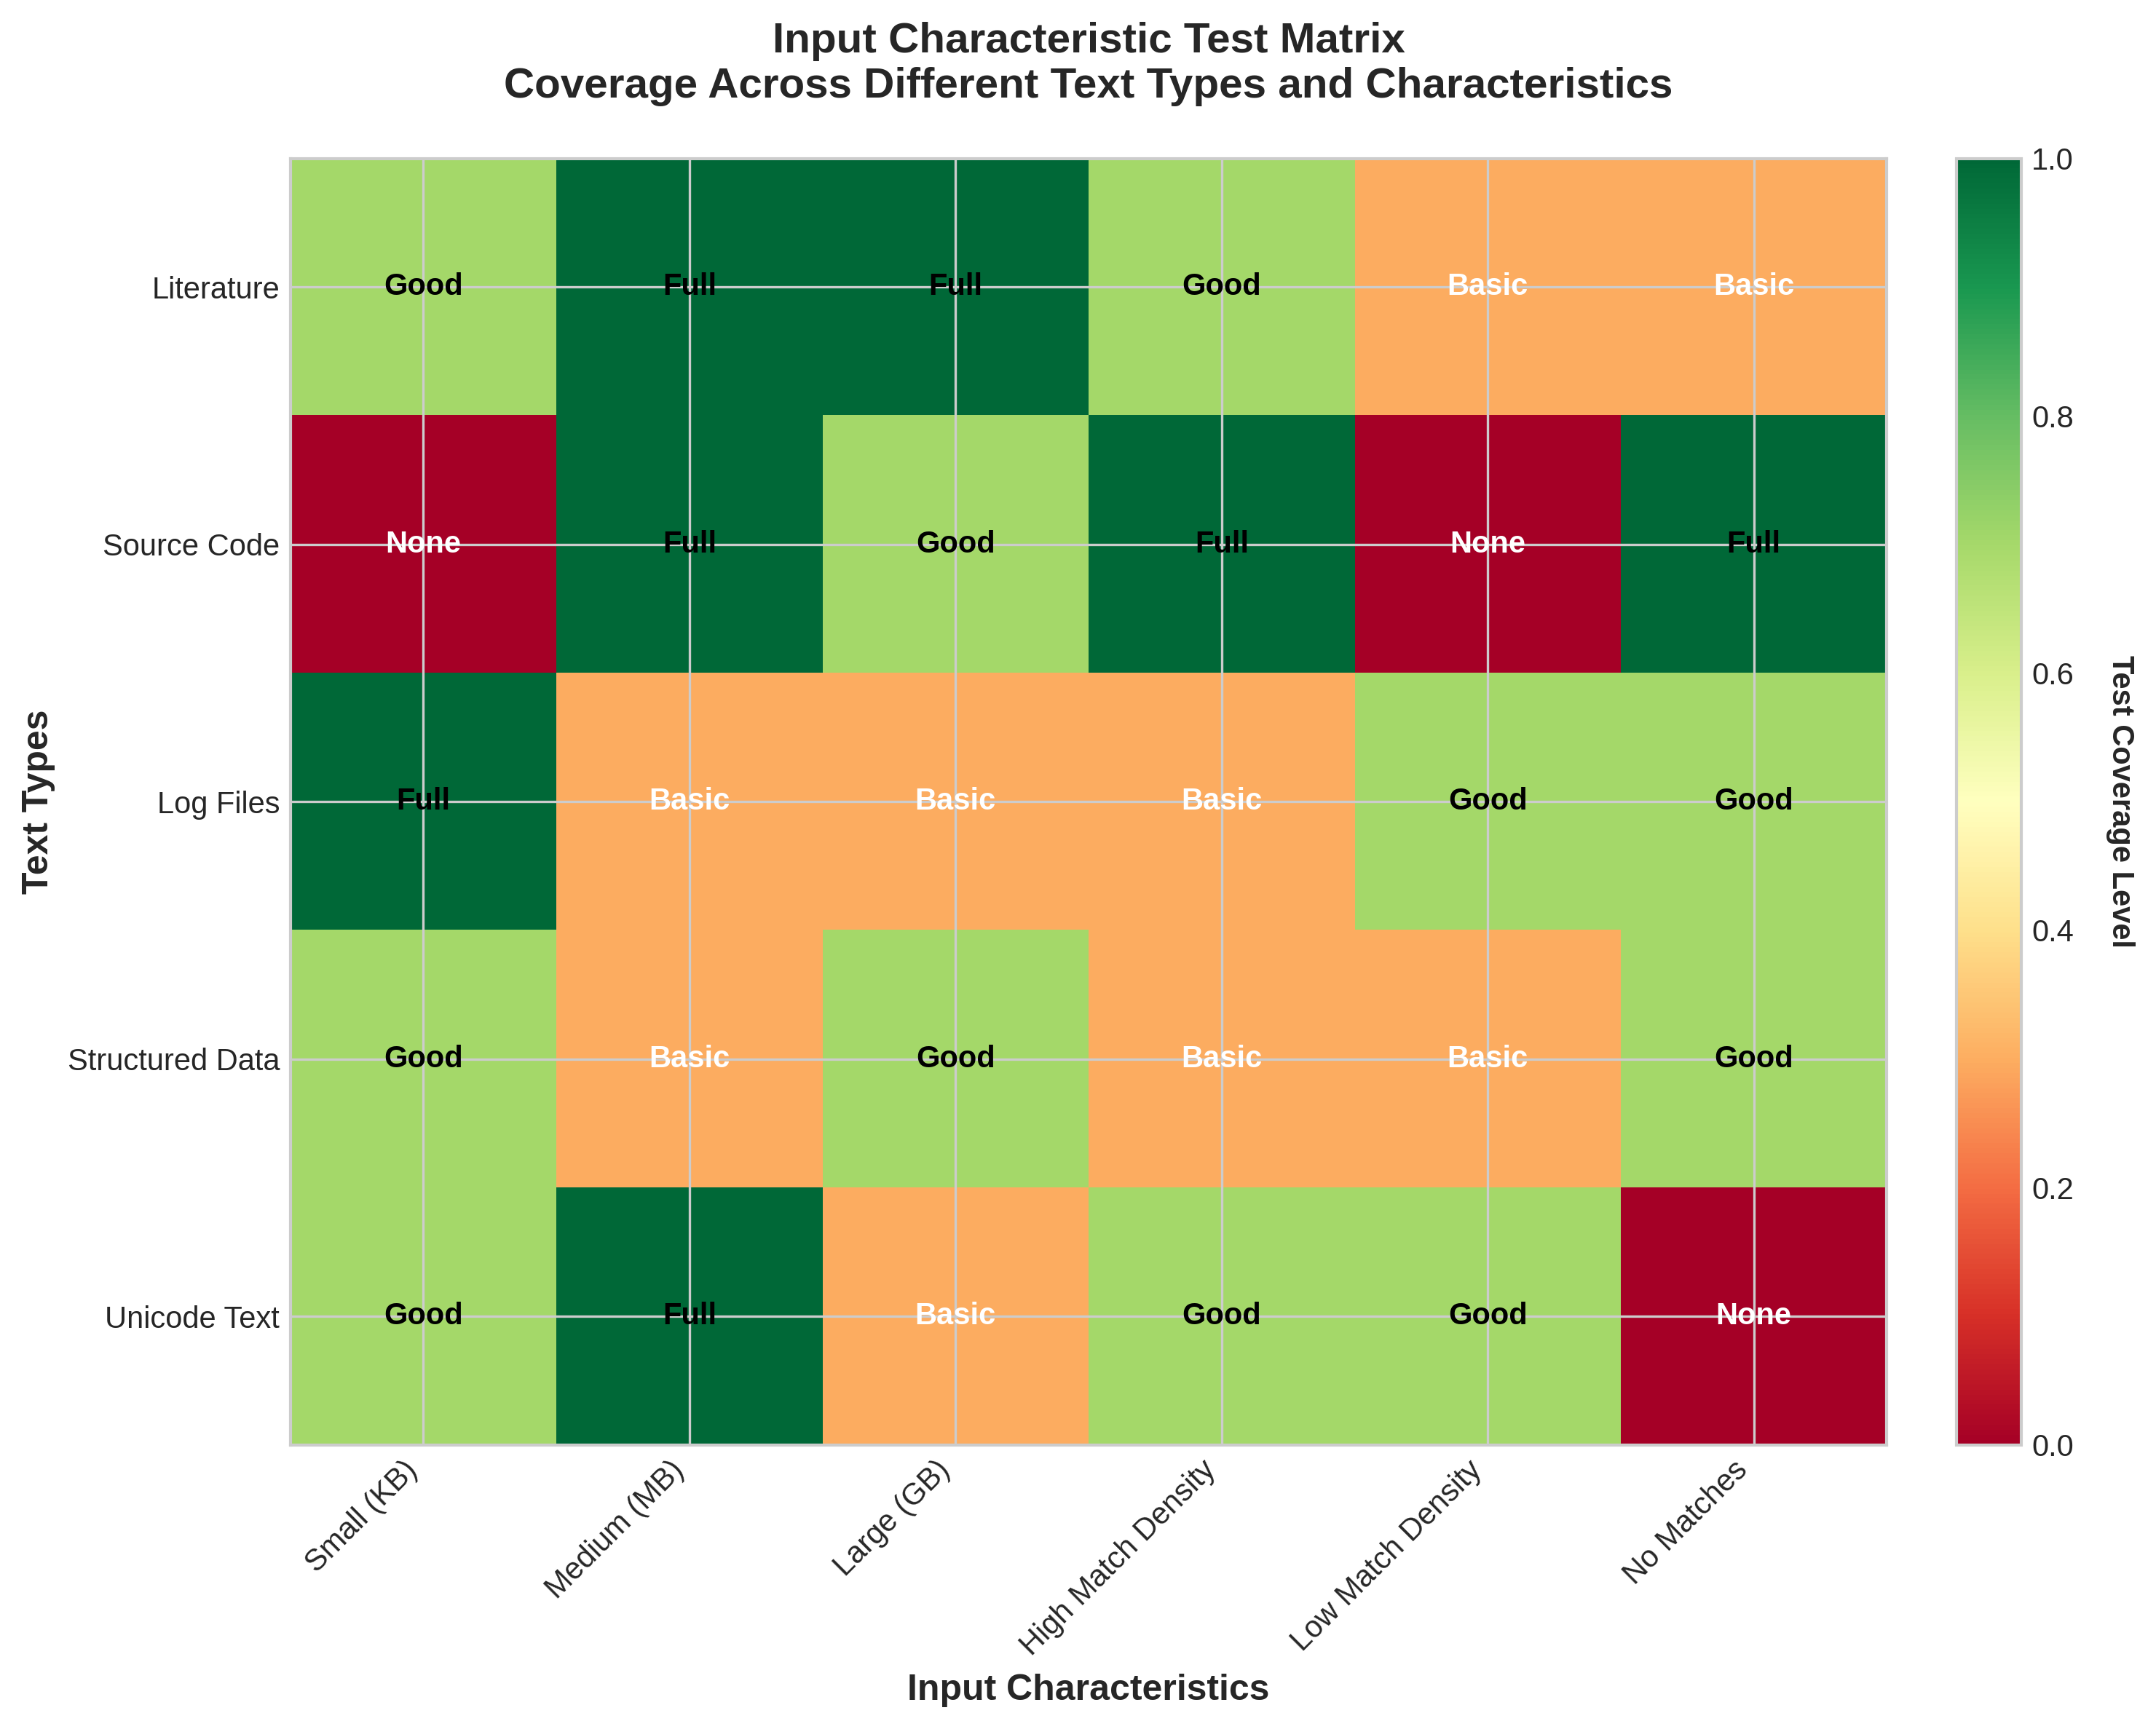
\includegraphics[width=0.8\textwidth]{illustrations/input_characteristics.png}
\caption{Input Characteristic Test Matrix}
\label{fig:input_characteristics}
\end{figure}

\begin{enumerate}
    \item \textbf{Text Structure Variation}: Different text types (code, natural language, structured data)
    \item \textbf{Match Density Scenarios}: High-match, low-match, and no-match scenarios
    \item \textbf{Input Size Scaling}: Testing performance across different input sizes
    \item \textbf{Unicode Complexity}: Various Unicode character sets and normalization scenarios
\end{enumerate}

\subsubsection{Scale and Concurrency Tests}

\begin{enumerate}
    \item \textbf{Pattern Set Size Scaling}: Testing with 1 to 100,000+ patterns
    \item \textbf{Concurrent Matching}: Multi-threaded performance characteristics
    \item \textbf{Memory Pressure Tests}: Performance under various memory constraints
    \item \textbf{Long-Running Scenarios}: Sustained performance over extended periods
\end{enumerate}

\subsection{Advanced Metrics Framework}

Beyond basic throughput and memory usage, we propose collecting detailed performance metrics:

\begin{table}[H]
\centering
\begin{tabular}{@{}lp{8cm}@{}}
\toprule
\textbf{Metric Category} & \textbf{Specific Metrics} \\
\midrule
Throughput & MB/s, patterns/s, matches/s, characters/s \\
Latency & P50, P95, P99 response times, worst-case latency \\
Memory & Peak usage, allocation rate, GC pressure, memory efficiency \\
CPU & CPU utilization, cache miss rates, instruction throughput \\
Scalability & Throughput vs. pattern count, memory vs. pattern count \\
Quality & Match accuracy, false positive/negative rates \\
\bottomrule
\end{tabular}
\caption{Comprehensive Performance Metrics}
\label{tab:metrics}
\end{table}

\subsection{Test Data Generation}

\begin{figure}[H]
\centering
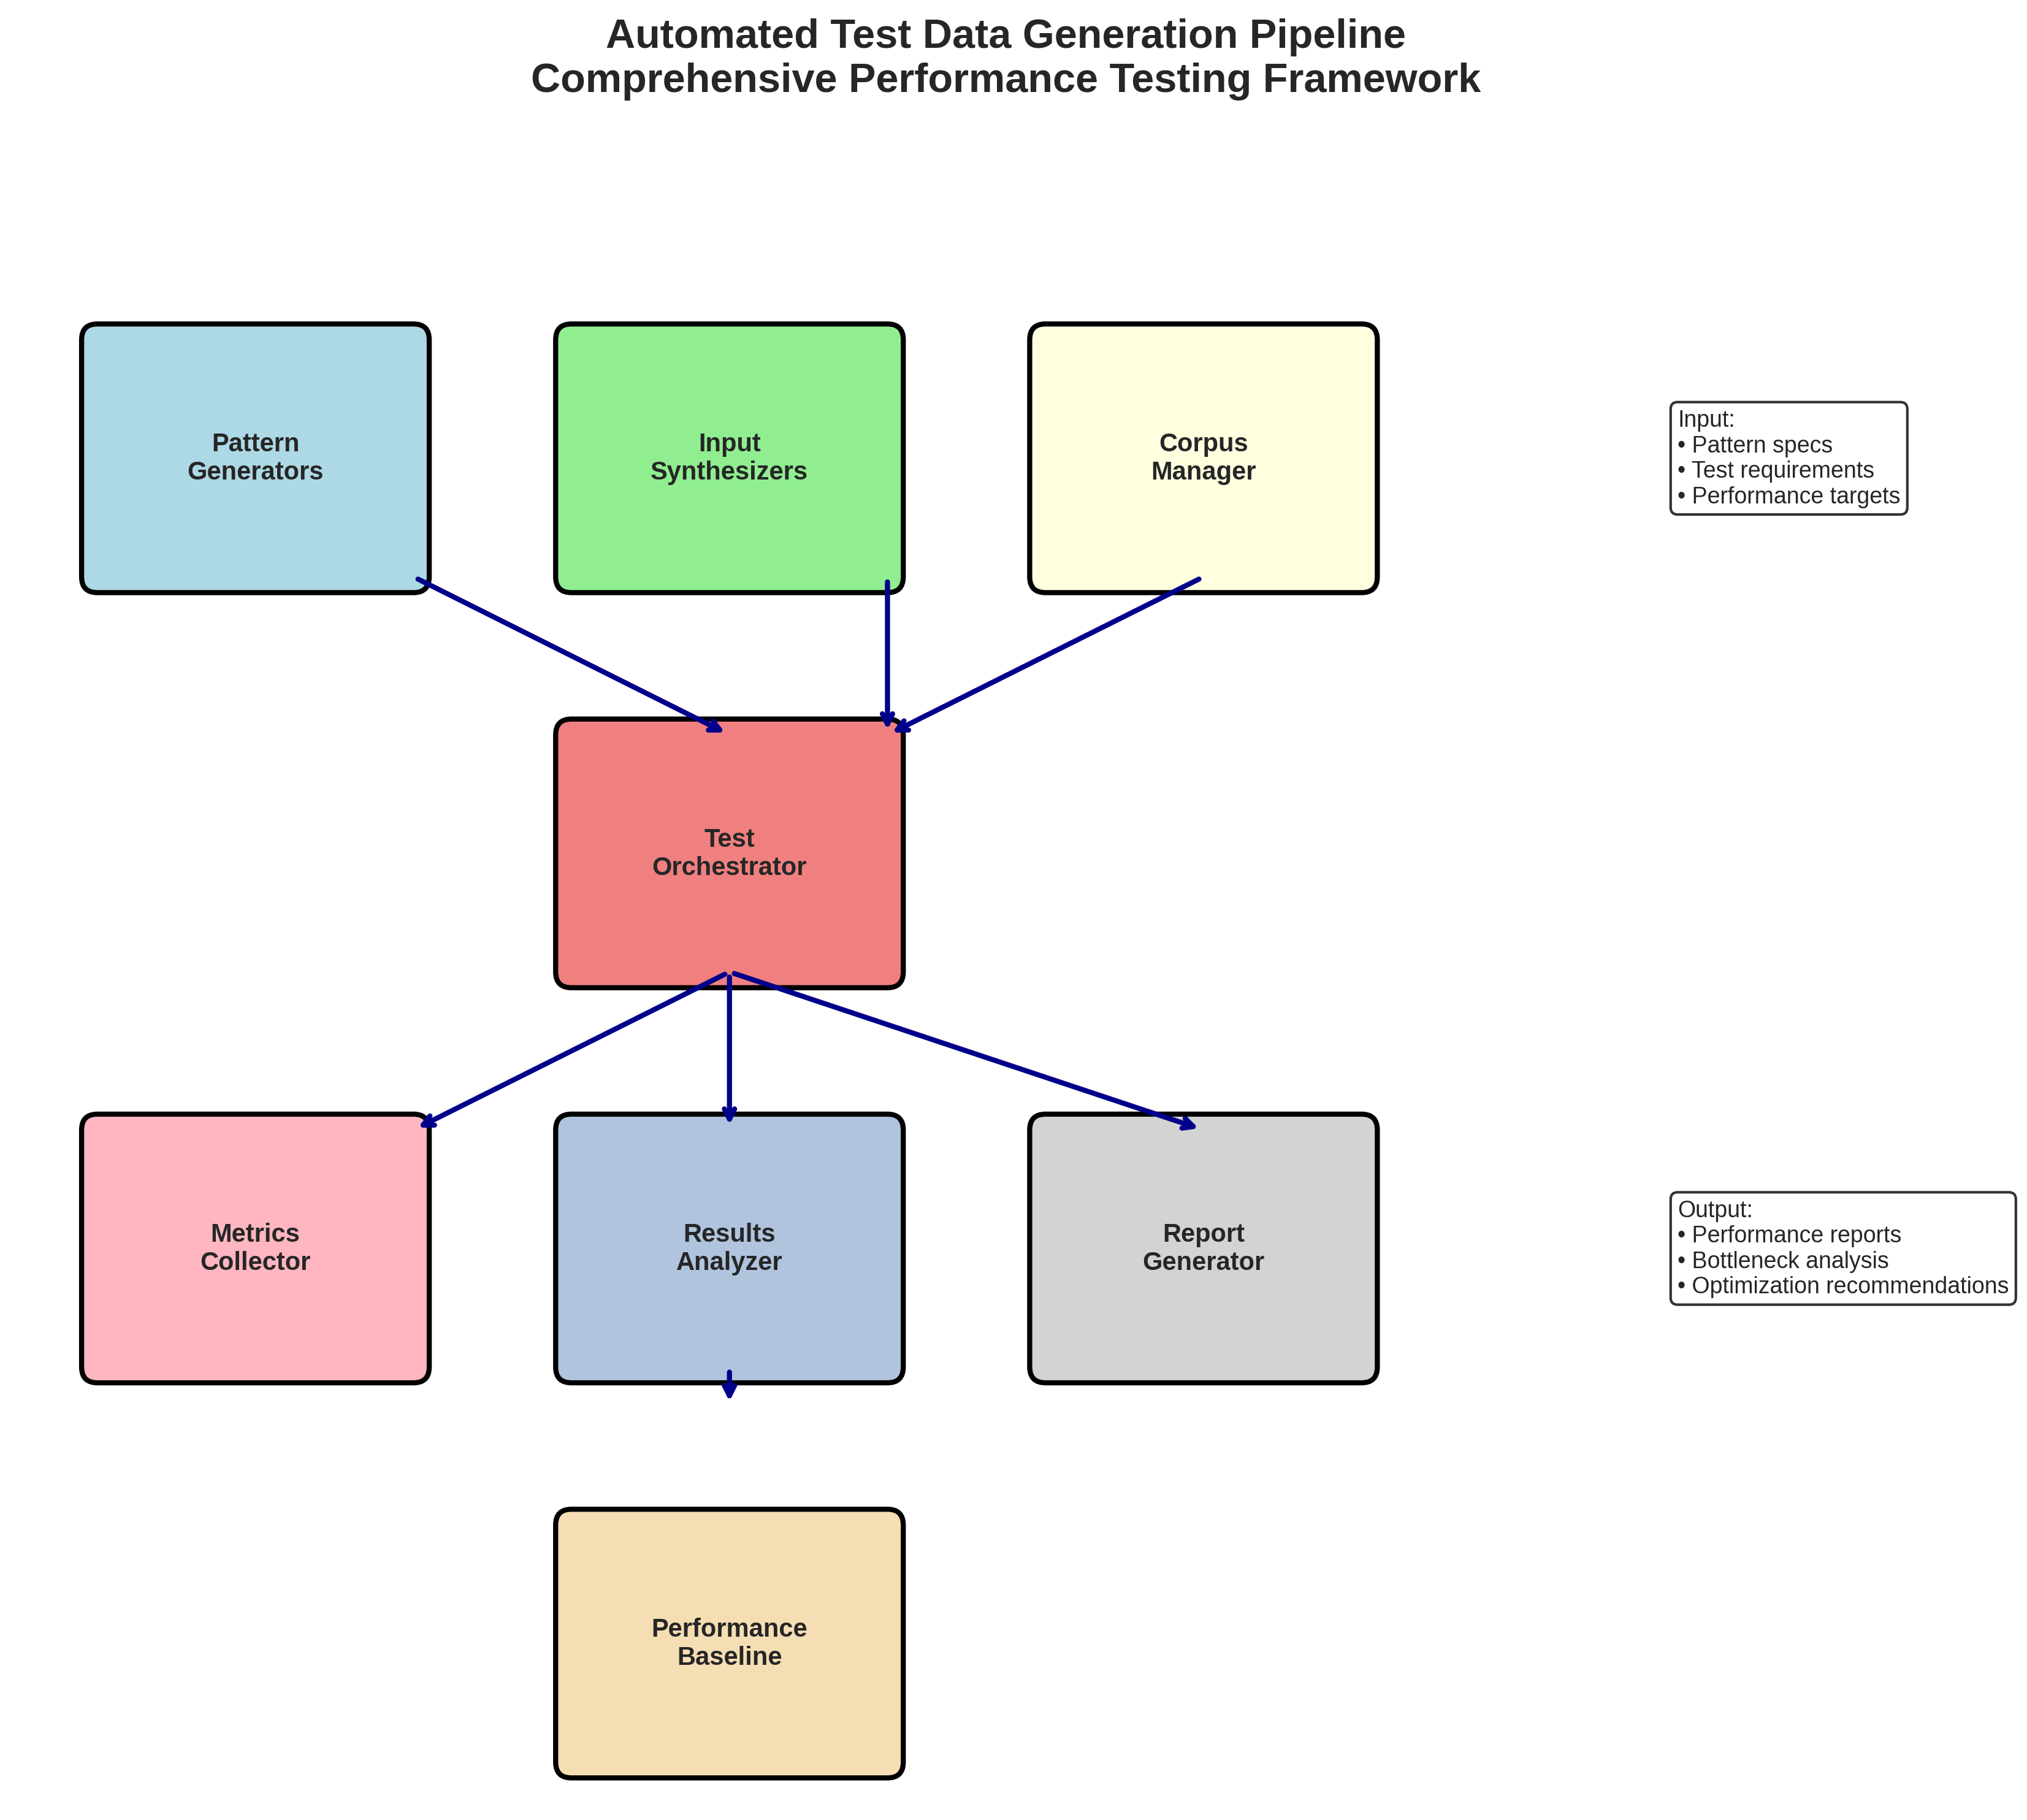
\includegraphics[width=0.9\textwidth]{illustrations/test_generation_pipeline.png}
\caption{Automated Test Data Generation Pipeline}
\label{fig:test_generation}
\end{figure}

We propose an automated test generation system that creates diverse test scenarios:

\begin{enumerate}
    \item \textbf{Pattern Generators}: Algorithmic generation of patterns with specific characteristics
    \item \textbf{Input Synthesizers}: Creation of synthetic inputs that stress different aspects of the engine
    \item \textbf{Corpus Diversification}: Automatic expansion of test corpora from various domains
    \item \textbf{Property-Based Testing}: Randomized testing with invariant checking
\end{enumerate}

\section{Implementation Architecture}

\subsection{Framework Components}

\begin{figure}[H]
\centering
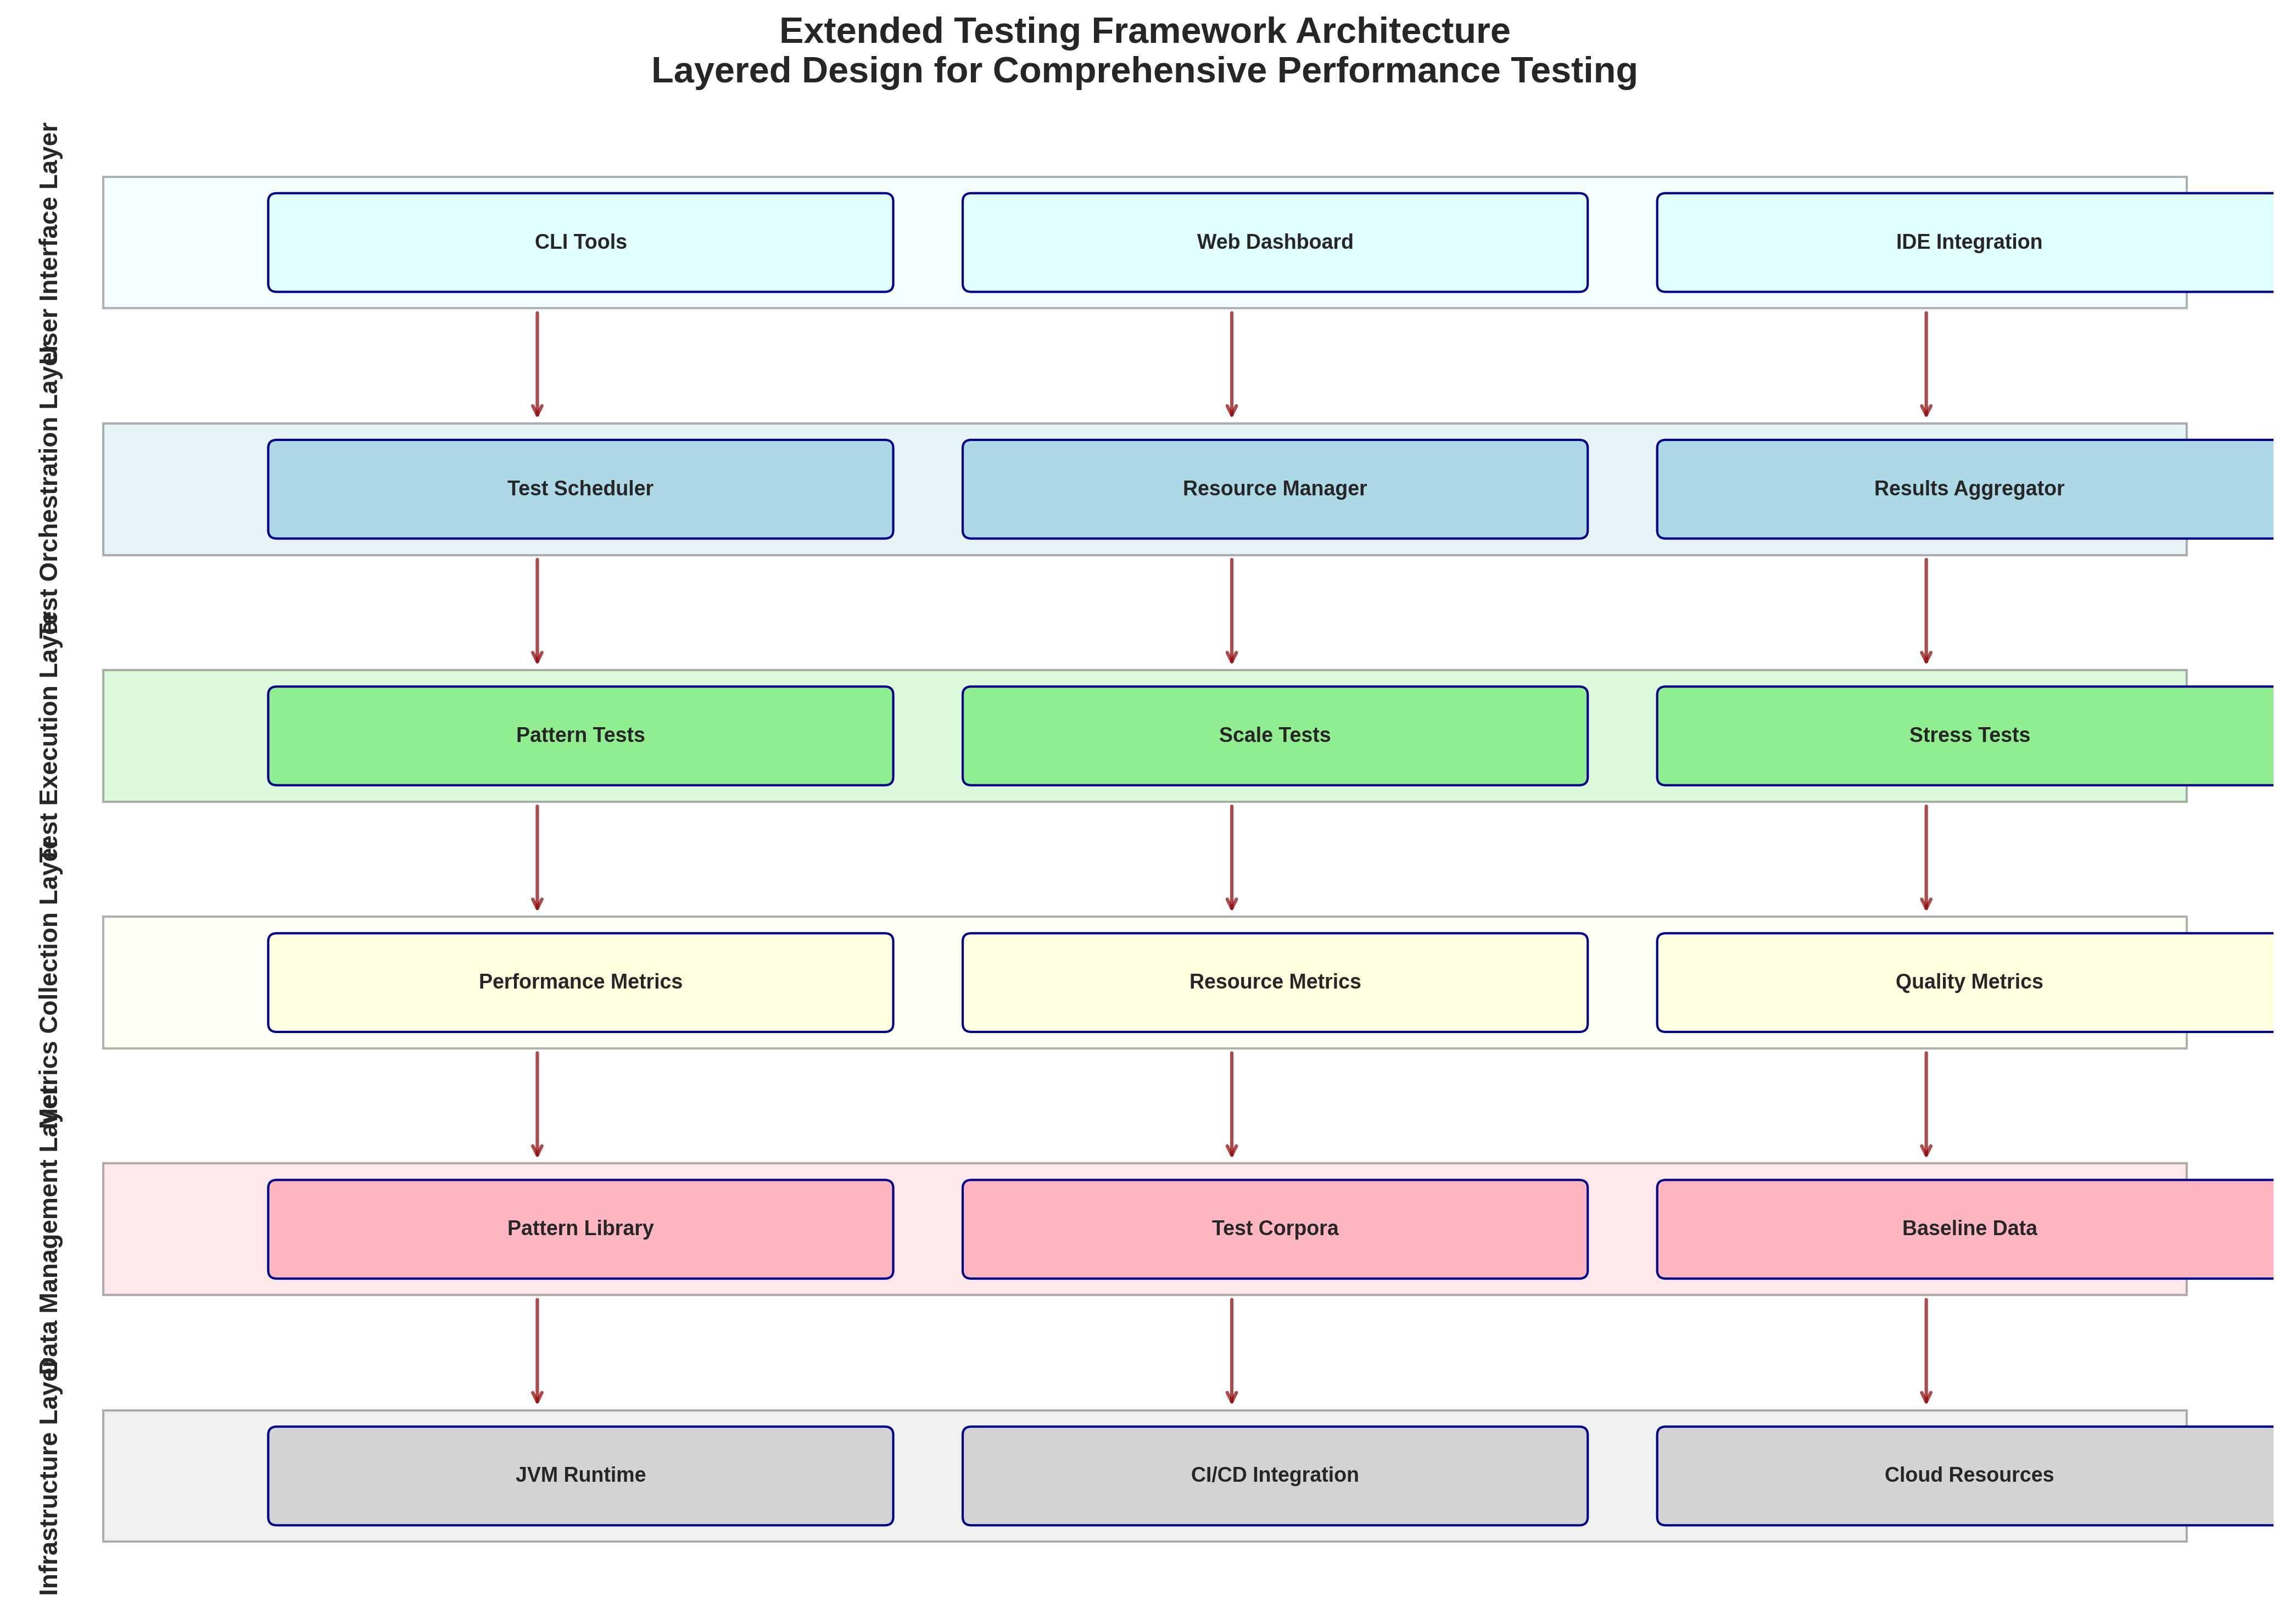
\includegraphics[width=0.9\textwidth]{illustrations/testing_architecture.png}
\caption{Extended Testing Framework Architecture}
\label{fig:architecture}
\end{figure}

The testing framework consists of several interconnected components:

\begin{enumerate}
    \item \textbf{Test Orchestrator}: Coordinates test execution and result collection
    \item \textbf{Pattern Library}: Curated collection of test patterns organized by category
    \item \textbf{Corpus Manager}: Manages diverse test input corpora
    \item \textbf{Metrics Collector}: Gathers comprehensive performance metrics
    \item \textbf{Results Analyzer}: Processes and interprets test results
    \item \textbf{Report Generator}: Creates actionable performance reports
\end{enumerate}

\subsection{Integration with Existing Infrastructure}

The extended testing framework integrates seamlessly with existing rmatch infrastructure:

\begin{itemize}
    \item Extends existing JMH benchmarks with new test scenarios
    \item Integrates with GitHub Actions for continuous performance monitoring
    \item Maintains compatibility with existing baseline management
    \item Provides migration path from current testing approaches
\end{itemize}

\section{Performance Insights and Optimization Guidance}

\subsection{Performance Characterization}

The extended testing regime will provide insights into:

\begin{figure}[H]
\centering
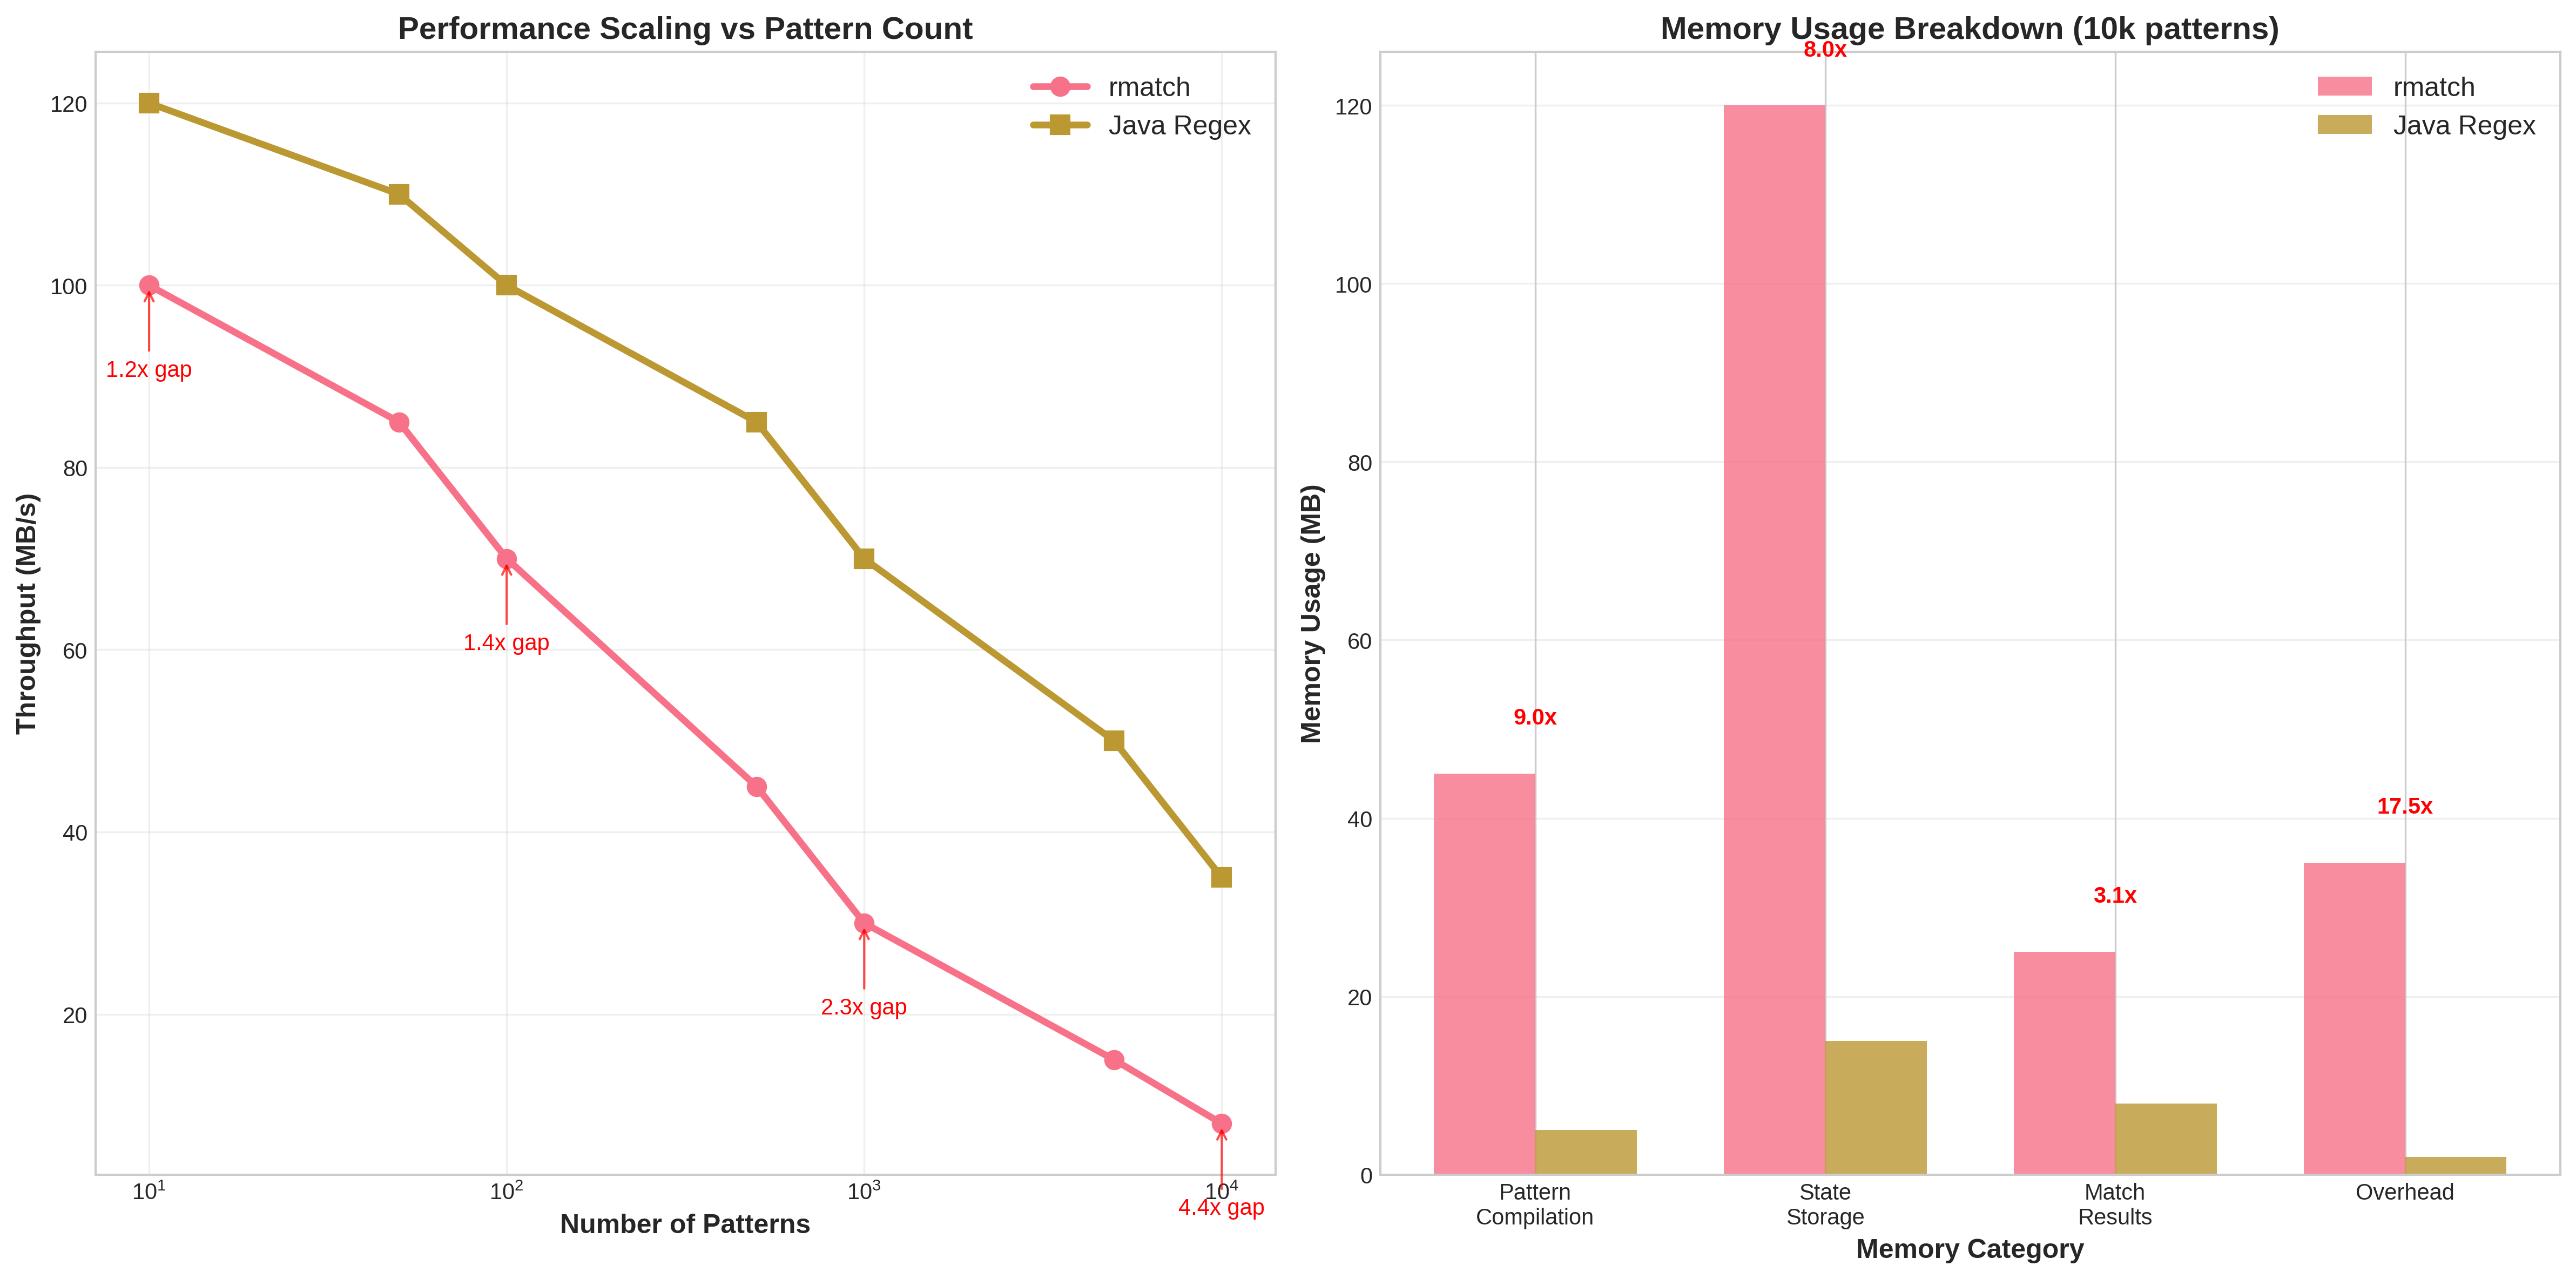
\includegraphics[width=0.8\textwidth]{illustrations/performance_characterization.png}
\caption{Performance Characterization Matrix}
\label{fig:performance_char}
\end{figure}

\begin{enumerate}
    \item \textbf{Algorithmic Complexity}: How performance scales with input and pattern complexity
    \item \textbf{Implementation Bottlenecks}: Specific code paths that limit performance
    \item \textbf{Resource Utilization}: Efficiency of CPU, memory, and cache usage
    \item \textbf{Trade-off Analysis}: Performance vs. memory vs. compilation time trade-offs
\end{enumerate}

\subsection{Optimization Prioritization}

Results from the extended testing will guide optimization efforts by:

\begin{itemize}
    \item Identifying scenarios where rmatch underperforms most significantly
    \item Revealing optimization opportunities with the highest impact potential
    \item Providing clear metrics for measuring optimization effectiveness
    \item Enabling data-driven decision making for algorithmic improvements
\end{itemize}

\section{Expected Benefits}

\subsection{Short-term Benefits}

\begin{itemize}
    \item Clear identification of current performance bottlenecks
    \item Validation of existing optimization hypotheses
    \item Improved confidence in performance claims
    \item Better understanding of competitive positioning vs. Java regex
\end{itemize}

\subsection{Long-term Benefits}

\begin{itemize}
    \item Systematic approach to performance optimization
    \item Reduced risk of performance regressions
    \item Enhanced ability to evaluate new algorithmic approaches
    \item Foundation for performance-driven development processes
\end{itemize}

\section{Implementation Timeline}

\begin{table}[H]
\centering
\begin{tabular}{@{}llp{6cm}@{}}
\toprule
\textbf{Phase} & \textbf{Duration} & \textbf{Deliverables} \\
\midrule
Phase 1 & 2-3 weeks & Test framework foundation, basic pattern library \\
Phase 2 & 3-4 weeks & Advanced metrics collection, test generation \\
Phase 3 & 2-3 weeks & CI/CD integration, automated reporting \\
Phase 4 & 2-3 weeks & Documentation, optimization guidance \\
\midrule
\textbf{Total} & \textbf{9-13 weeks} & \textbf{Complete extended testing regime} \\
\bottomrule
\end{tabular}
\caption{Implementation Timeline}
\label{tab:timeline}
\end{table}

\section{Risk Mitigation}

\subsection{Technical Risks}

\begin{itemize}
    \item \textbf{Test Execution Time}: Mitigate with parallel execution and test prioritization
    \item \textbf{Result Interpretation Complexity}: Provide clear guidelines and automated analysis
    \item \textbf{Maintenance Overhead}: Design for modularity and automated maintenance
\end{itemize}

\subsection{Organizational Risks}

\begin{itemize}
    \item \textbf{Resource Requirements}: Implement incrementally to manage resource usage
    \item \textbf{Adoption Resistance}: Provide clear value demonstration and migration support
    \item \textbf{Tool Complexity}: Ensure user-friendly interfaces and comprehensive documentation
\end{itemize}

\section{Conclusion}

The proposed extended testing regime addresses critical limitations in the current rmatch testing infrastructure. By providing comprehensive, diverse, and automated testing scenarios, it will enable more effective performance optimization and provide clearer guidance for development priorities.

The framework's modular design ensures compatibility with existing infrastructure while providing a foundation for systematic performance improvement efforts. Implementation can proceed incrementally, providing immediate value while building toward the complete testing regime.

\appendix

\section{Task Implementation Guide}

This appendix provides detailed task descriptions for implementing the extended testing regime through the GitHub agent. Each task is designed to be self-contained and executable in sequence.

\subsection{Task 001: Foundation Infrastructure}

\subsubsection{Title}
Set up Extended Testing Framework Foundation

\subsubsection{Problem}
The current testing infrastructure has critical foundational issues that must be addressed before comprehensive performance testing can be implemented effectively. Specifically, the system still relies on legacy CSV logging mechanisms instead of modern JMH infrastructure, creating inconsistencies and limiting GitHub Actions compatibility.

\subsubsection{Proposal}
Modernize and establish the foundational infrastructure for the extended testing framework:
\begin{itemize}
    \item \textbf{Remove legacy CSV logging infrastructure}: Deprecate and eliminate \texttt{CSVAppender} class and all CSV-based measurements to ensure consistency~\cite{jmh2013}
    \item \textbf{Standardize on JMH infrastructure}: Migrate all performance measurements to use the existing JMH framework for accuracy and GitHub Actions compatibility
    \item \textbf{Establish modern test framework architecture}: Create JMH-integrated components for test orchestration and pattern management
    \item \textbf{Implement enhanced metrics collection framework}: Extend JMH-based metrics to include latency percentiles and advanced performance indicators
\end{itemize}

\subsubsection{Alternatives}
\begin{enumerate}
    \item \textbf{Build entirely new testing framework}: Clean design but high effort and potential compatibility issues with existing baseline management
    \item \textbf{Extend existing JMH infrastructure (Recommended)}: Lower effort, maintains compatibility with current performance evaluation systems~\cite{blackburn2006dacapo}, and ensures GitHub Actions compatibility~\cite{github_actions}
    \item \textbf{Hybrid approach}: Combine new components with existing infrastructure, providing balanced effort and benefits while enabling gradual migration from legacy systems
\end{enumerate}

\subsection{Task 001E: Foundation Infrastructure Evaluation \& Learning}

\subsubsection{Title}
Evaluate Foundation Infrastructure Implementation and Capture Learning

\subsubsection{Problem}
Implementation experience from Task 001 needs to be captured and analyzed to inform subsequent task planning and design decisions. Lessons learned about JMH integration complexity, infrastructure modernization challenges, and performance impact need to be documented and incorporated into future task specifications.

\subsubsection{Proposal}
Conduct comprehensive evaluation of the foundation infrastructure implementation:
\begin{itemize}
    \item \textbf{Performance Impact Assessment}: Measure actual overhead of new framework components vs. baseline expectations
    \item \textbf{Integration Complexity Analysis}: Document challenges encountered during JMH modernization and CSV system removal
    \item \textbf{Design Decision Validation}: Evaluate effectiveness of chosen architecture patterns for extensibility and maintainability
    \item \textbf{Learning Capture \& Plan Refinement}: Update subsequent task descriptions based on implementation insights and performance characteristics discovered
\end{itemize}

\subsubsection{Learning Questions \& Reflection Points}
\begin{enumerate}
    \item \textbf{JMH Integration}: Was the CSV-to-JMH migration smoother or more complex than anticipated? What specific technical challenges emerged?
    \item \textbf{Performance Baseline}: How does the new framework compare to legacy CSV-based measurements in terms of accuracy and overhead?
    \item \textbf{GitHub Actions Compatibility}: Are there unexpected CI/CD integration issues that should inform Task 005 planning?
    \item \textbf{Architecture Decisions}: Which design patterns worked well and which should be reconsidered for subsequent tasks?
\end{enumerate}

\subsubsection{Plan Refinement Actions}
Based on evaluation results, update subsequent task specifications:
\begin{itemize}
    \item Adjust complexity estimates for Tasks 002-008 based on actual infrastructure modernization effort
    \item Refine performance testing approaches in Task 004 based on discovered JMH capabilities and limitations
    \item Update CI/CD integration strategy in Task 005 based on GitHub Actions compatibility findings
    \item Modify documentation requirements in Task 008 based on implementation complexity insights
\end{itemize}

% LEARNING COMMENTS: This space reserved for capturing actual implementation insights
% TODO: After Task 001 completion, update this section with:
% - Specific technical challenges encountered
% - Performance impact measurements vs. expectations
% - Architecture decisions that should influence subsequent tasks
% - Refined effort estimates for remaining tasks

\subsection{Task 002: Pattern Library Development}

\subsubsection{Title}
Develop Comprehensive Test Pattern Library

\subsubsection{Problem}
Current tests use limited pattern sets that don't represent the diversity of real-world regex usage. We need a comprehensive library of test patterns covering different complexity categories.

\subsubsection{Proposal}
Create a structured pattern library with:
\begin{itemize}
    \item Categorized pattern collections (simple, complex, pathological)
    \item Pattern metadata including complexity metrics
    \item Automated pattern generation capabilities
    \item Pattern validation and correctness verification
\end{itemize}

\subsubsection{Alternatives}
\begin{enumerate}
    \item Manual curation of patterns (high quality, labor intensive)
    \item Automated generation with manual validation (scalable, requires validation)
    \item Crowd-sourced pattern collection (diverse, quality control challenges)
\end{enumerate}

\subsection{Task 002E: Pattern Library Evaluation \& Learning}

\subsubsection{Title}
Evaluate Pattern Library Implementation and Refine Testing Strategy

\subsubsection{Problem}
Pattern library implementation provides critical insights into pattern complexity characteristics, automated generation effectiveness, and performance impact across different pattern categories. These learnings must inform subsequent corpus diversification and metrics collection strategies.

\subsubsection{Proposal}
Conduct comprehensive evaluation of pattern library implementation:
\begin{itemize}
    \item \textbf{Pattern Coverage Analysis}: Assess completeness and quality of generated patterns across complexity categories
    \item \textbf{Performance Characterization}: Measure actual performance impact of different pattern types vs. theoretical complexity metrics
    \item \textbf{Generation System Effectiveness}: Evaluate automated pattern generation quality and manual validation effort required
    \item \textbf{Integration Assessment}: Test pattern library integration with Task 001 infrastructure for scalability and maintainability
\end{itemize}

\subsubsection{Learning Questions \& Reflection Points}
\begin{enumerate}
    \item \textbf{Pattern Quality}: Did automated generation produce realistic and valuable test patterns, or is manual curation more critical than anticipated?
    \item \textbf{Complexity Metrics}: How well do theoretical complexity scores correlate with actual rmatch performance characteristics?
    \item \textbf{Coverage Gaps}: What regex features or pattern types are still under-represented and should be prioritized?
    \item \textbf{Performance Insights}: Which pattern categories revealed unexpected performance characteristics that should influence algorithm development?
\end{enumerate}

\subsubsection{Plan Refinement Actions}
Based on pattern library evaluation, update subsequent task planning:
\begin{itemize}
    \item Adjust input corpus selection in Task 003 to prioritize text domains that complement discovered pattern performance characteristics
    \item Refine metrics collection in Task 004 to focus on performance dimensions revealed as most critical by pattern analysis
    \item Update automated test generation in Task 005 to incorporate pattern effectiveness learnings
    \item Modify optimization guidance in Task 007 based on performance bottlenecks identified through pattern library testing
\end{itemize}

% LEARNING COMMENTS: This space reserved for capturing pattern library implementation insights
% TODO: After Task 002 completion, update this section with:
% - Pattern generation quality assessment and refinement recommendations
% - Correlation analysis between complexity metrics and actual performance
% - Specific pattern categories that revealed optimization opportunities
% - Revised estimates for corpus selection and metrics collection priorities

\subsection{Task 003: Input Corpus Diversification}

\subsubsection{Title}
Expand Test Input Corpus Beyond Wuthering Heights

\subsubsection{Problem}
Testing primarily on a single literary text limits the generalizability of performance results. Different text types may reveal different performance characteristics.

\subsubsection{Proposal}
Develop a diverse corpus collection including bioinformatics datasets and established benchmarks:
\begin{itemize}
    \item \textbf{Bioinformatics Data}: DNA/RNA sequences from NCBI GenBank~\cite{ncbi_genbank}, protein sequences from UniProt~\cite{uniprot2021}, and genome annotations from Ensembl~\cite{cunningham2022ensembl}
    \item \textbf{Established Benchmarks}: Canterbury Corpus~\cite{canterbury_corpus} and Large Text Compression Benchmark~\cite{large_text_benchmark} for standardized comparisons
    \item \textbf{Multiple text domains}: Literature, source code, log files, structured data, and social media text
    \item \textbf{Various text characteristics}: Different character sets, line lengths, and structural patterns
    \item \textbf{Synthetic input generation}: Controlled stress testing with known pattern matching properties
    \item \textbf{Comprehensive metadata}: Domain-specific annotations for result interpretation and pattern complexity analysis
\end{itemize}

The bioinformatics datasets are particularly valuable because they represent real-world pattern matching scenarios with high repetition rates, long exact matches, and biological motifs that stress different aspects of regex engines compared to literary text. Integration with established benchmark collections ensures compatibility with broader pattern matching research~\cite{altschul1990basic,gusfield1997algorithms}.

\subsubsection{Alternatives}
\begin{enumerate}
    \item \textbf{Use existing public corpora}: Quick setup with established datasets like Canterbury Corpus~\cite{canterbury_corpus}, but may not cover rmatch-specific needs and requires careful licensing consideration
    \item \textbf{Generate all synthetic corpora}: Provides controlled characteristics and unlimited variety, but may not reflect real-world usage patterns found in biological sequences or established benchmarks
    \item \textbf{Hybrid real + synthetic approach (Recommended)}: Combines realistic patterns from bioinformatics datasets~\cite{durbin1998biological} with controlled testing scenarios, providing both validation against known benchmarks and stress testing capabilities
    \item \textbf{Community-contributed corpora}: Leverages diverse real-world inputs and community engagement, but requires quality control and careful handling of privacy/licensing issues
\end{enumerate}

\subsection{Task 003E: Input Corpus Evaluation \& Learning}

\subsubsection{Title}
Evaluate Corpus Diversification Impact and Refine Performance Understanding

\subsubsection{Problem}
Corpus diversification reveals how rmatch performance varies across different text domains and characteristics. These insights are critical for understanding optimization priorities and developing appropriate metrics collection strategies for Task 004.

\subsubsection{Proposal}
Conduct comprehensive evaluation of corpus diversification impact:
\begin{itemize}
    \item \textbf{Domain-Specific Performance Analysis}: Compare rmatch performance across literary, bioinformatics, code, and log file domains
    \item \textbf{Text Characteristic Impact Assessment}: Measure how factors like character set diversity, line length, and structural patterns affect performance
    \item \textbf{Bioinformatics Dataset Insights}: Analyze performance on biological sequences to understand long exact match and high repetition scenarios
    \item \textbf{Benchmark Comparison Validation}: Validate rmatch results against established benchmark collections for research credibility
\end{itemize}

\subsubsection{Learning Questions \& Reflection Points}
\begin{enumerate}
    \item \textbf{Domain Variations}: Which text domains revealed unexpected performance characteristics that differ from literary text assumptions?
    \item \textbf{Bioinformatics Performance}: Do biological sequences stress rmatch differently than anticipated, requiring algorithm adjustments?
    \item \textbf{Optimization Priorities}: Which corpus characteristics suggest the most impactful optimization directions?
    \item \textbf{Metrics Requirements}: What performance dimensions became critical across diverse corpora that weren't apparent with single-domain testing?
\end{enumerate}

\subsubsection{Plan Refinement Actions}
Based on corpus evaluation insights, refine subsequent task approaches:
\begin{itemize}
    \item Prioritize specific latency/throughput metrics in Task 004 based on domain-specific performance variations discovered
    \item Adjust automated test generation in Task 005 to focus on corpus characteristics that revealed optimization opportunities
    \item Update CI/CD integration in Task 006 to emphasize performance monitoring for most critical text domains
    \item Refine optimization guidance in Task 007 based on domain-specific bottlenecks identified
\end{itemize}

% LEARNING COMMENTS: This space reserved for capturing corpus diversification insights
% TODO: After Task 003 completion, update this section with:
% - Specific domain performance variations and their implications
% - Bioinformatics dataset insights and algorithm stress points
% - Text characteristic factors most impactful on rmatch performance
% - Refined metrics collection priorities based on cross-domain analysis

\subsection{Task 004: Advanced Metrics Collection}

\subsubsection{Title}
Implement Comprehensive Performance Metrics Collection

\subsubsection{Problem}
Current metrics focus on basic throughput and memory usage. More detailed metrics are needed to understand performance characteristics and guide optimization efforts.

\subsubsection{Proposal}
Extend metrics collection to include:
\begin{itemize}
    \item Latency percentiles (P50, P95, P99)
    \item CPU utilization and cache performance
    \item Detailed memory allocation patterns
    \item Scalability metrics across different dimensions
\end{itemize}

\subsubsection{Alternatives}
\begin{enumerate}
    \item Use JVM profiling tools (detailed but complex)
    \item Implement custom metrics collection (tailored but requires development)
    \item Integrate with monitoring platforms (comprehensive but adds dependencies)
\end{enumerate}

\subsection{Task 004E: Advanced Metrics Evaluation \& Learning}

\subsubsection{Title}
Evaluate Advanced Metrics Implementation and Refine Performance Understanding

\subsubsection{Problem}
Advanced metrics collection reveals the detailed performance characteristics necessary for effective optimization guidance. The implementation provides insights into which metrics are most valuable for identifying bottlenecks and guiding development priorities.

\subsubsection{Proposal}
Conduct comprehensive evaluation of advanced metrics implementation:
\begin{itemize}
    \item \textbf{Metrics Effectiveness Assessment}: Evaluate which metrics provide the most actionable insights for optimization decisions
    \item \textbf{Collection Overhead Analysis}: Measure performance impact of metrics collection itself across different monitoring intensities
    \item \textbf{Bottleneck Identification Validation}: Test effectiveness of new metrics for identifying actual performance bottlenecks vs. baseline throughput measurements
    \item \textbf{Cross-Domain Metrics Analysis}: Analyze metric behavior across diverse corpora from Task 003 to understand domain-specific optimization priorities
\end{itemize}

\subsubsection{Learning Questions \& Reflection Points}
\begin{enumerate}
    \item \textbf{Critical Metrics}: Which latency percentiles and performance dimensions proved most valuable for identifying optimization opportunities?
    \item \textbf{Collection Trade-offs}: What is the optimal balance between metrics detail and collection overhead for continuous monitoring?
    \item \textbf{Domain Sensitivity}: How do optimal metrics vary across different text domains and pattern complexities?
    \item \textbf{Actionability}: Which metrics translate most directly to specific optimization strategies and algorithm improvements?
\end{enumerate}

\subsubsection{Plan Refinement Actions}
Based on metrics evaluation insights, optimize subsequent task strategies:
\begin{itemize}
    \item Focus automated test generation in Task 005 on scenarios that exercise the most critical performance dimensions identified
    \item Configure CI/CD integration in Task 006 to emphasize the most actionable metrics for regression detection
    \item Prioritize analysis and reporting in Task 007 around metrics that proved most effective for optimization guidance
    \item Update documentation in Task 008 to emphasize metrics interpretation patterns discovered through implementation
\end{itemize}

% LEARNING COMMENTS: This space reserved for capturing advanced metrics implementation insights
% TODO: After Task 004 completion, update this section with:
% - Ranking of metric effectiveness for optimization guidance
% - Optimal collection overhead vs. insight trade-offs
% - Domain-specific metric sensitivity patterns
% - Specific bottleneck identification success stories and refinements needed

\subsection{Task 005: Automated Test Generation}

\subsubsection{Title}
Develop Automated Test Case Generation System

\subsubsection{Problem}
Manual test case creation is time-consuming and may miss important edge cases. Automated generation can provide broader coverage and stress testing capabilities.

\subsubsection{Proposal}
Implement automated test generation including:
\begin{itemize}
    \item Pattern generation with specific complexity characteristics
    \item Input synthesis for targeted performance testing
    \item Property-based testing with invariant checking
    \item Randomized stress testing scenarios
\end{itemize}

\subsubsection{Alternatives}
\begin{enumerate}
    \item Rule-based generation (predictable but limited creativity)
    \item Machine learning-based generation (innovative but complex)
    \item Genetic algorithm approach (explores space well but unpredictable)
\end{enumerate}

\subsection{Task 005E: Automated Test Generation Evaluation \& Learning}

\subsubsection{Title}
Evaluate Automated Test Generation Effectiveness and Refine Testing Strategy

\subsubsection{Problem}
Automated test generation provides insights into edge cases, stress scenarios, and pattern combinations that manual testing might miss. The effectiveness of different generation strategies must be evaluated to optimize testing coverage and integration with CI/CD workflows.

\subsubsection{Proposal}
Conduct comprehensive evaluation of automated test generation implementation:
\begin{itemize}
    \item \textbf{Coverage Effectiveness Assessment}: Measure how automated generation improves test coverage beyond manual pattern curation
    \item \textbf{Edge Case Discovery Analysis}: Evaluate effectiveness of different generation strategies for identifying performance edge cases and correctness issues
    \item \textbf{Generation Strategy Comparison}: Compare rule-based, ML-based, and genetic algorithm approaches for practical testing value
    \item \textbf{Integration Readiness Evaluation}: Assess automated generation suitability for CI/CD integration and continuous testing workflows
\end{itemize}

\subsubsection{Learning Questions \& Reflection Points}
\begin{enumerate}
    \item \textbf{Generation Quality}: Which automated generation strategies produced the most valuable test cases for revealing rmatch performance characteristics?
    \item \textbf{Edge Case Value}: Did automated generation discover performance edge cases or correctness issues that manual testing missed?
    \item \textbf{Maintenance Requirements}: What is the ongoing effort required to maintain and tune automated generation vs. manual test case development?
    \item \textbf{CI/CD Readiness}: How should automated generation be integrated into continuous testing to provide maximum value without excessive execution time?
\end{enumerate}

\subsubsection{Plan Refinement Actions}
Based on automated generation evaluation, optimize CI/CD and reporting strategies:
\begin{itemize}
    \item Configure CI/CD integration in Task 006 to emphasize the most effective automated generation strategies
    \item Focus analysis and reporting in Task 007 on performance dimensions where automated generation revealed critical insights
    \item Update documentation in Task 008 to include best practices for automated test case interpretation and maintenance
    \item Adjust timeline estimates for ongoing maintenance based on generation strategy effectiveness findings
\end{itemize}

% LEARNING COMMENTS: This space reserved for capturing automated test generation insights
% TODO: After Task 005 completion, update this section with:
% - Comparative effectiveness of different generation strategies
% - Specific edge cases discovered through automation vs. manual testing
% - Integration complexity and maintenance requirements assessment
% - Recommendations for CI/CD integration and execution scheduling

\subsection{Task 006: CI/CD Integration}

\subsubsection{Title}
Integrate Extended Testing with GitHub Actions

\subsubsection{Problem}
Extended testing needs to be integrated into the development workflow to provide continuous performance monitoring and prevent regressions.

\subsubsection{Proposal}
Implement CI/CD integration with:
\begin{itemize}
    \item Automated test execution on pull requests
    \item Performance regression detection
    \item Baseline management and updating
    \item Automated performance reporting
\end{itemize}

\subsubsection{Alternatives}
\begin{enumerate}
    \item Run all tests on every commit (comprehensive but slow)
    \item Tiered testing approach (fast tests always, extended tests periodically)
    \item Manual trigger for extended tests (flexible but requires discipline)
\end{enumerate}

\subsection{Task 006E: CI/CD Integration Evaluation \& Learning}

\subsubsection{Title}
Evaluate CI/CD Integration Effectiveness and Refine Continuous Testing Strategy

\subsubsection{Problem}
CI/CD integration is critical for making the extended testing framework valuable in practice. The implementation provides insights into execution time trade-offs, regression detection effectiveness, and developer workflow integration that must inform final reporting and documentation strategies.

\subsubsection{Proposal}
Conduct comprehensive evaluation of CI/CD integration implementation:
\begin{itemize}
    \item \textbf{Execution Time Analysis}: Measure actual CI/CD execution times vs. targets for different testing tier configurations
    \item \textbf{Regression Detection Effectiveness}: Evaluate accuracy and sensitivity of automated performance regression detection across diverse scenarios
    \item \textbf{Developer Workflow Impact}: Assess integration smoothness and developer feedback on testing workflow changes
    \item \textbf{Baseline Management Evaluation}: Test effectiveness of automated baseline updating and performance trend tracking
\end{itemize}

\subsubsection{Learning Questions \& Reflection Points}
\begin{enumerate}
    \item \textbf{Execution Efficiency}: Did the tiered testing approach achieve the desired balance between comprehensiveness and speed?
    \item \textbf{Regression Sensitivity}: Are the performance gates appropriately tuned to catch meaningful regressions without false positives?
    \item \textbf{Adoption Barriers}: What aspects of the CI/CD integration create friction for developers and how can they be addressed?
    \item \textbf{Maintenance Overhead}: What ongoing maintenance requirements emerged for baseline management and test configuration?
\end{enumerate}

\subsubsection{Plan Refinement Actions}
Based on CI/CD integration evaluation, finalize framework implementation:
\begin{itemize}
    \item Optimize analysis and reporting in Task 007 based on CI/CD execution time constraints and developer feedback needs
    \item Focus documentation in Task 008 on addressing adoption barriers and workflow integration challenges identified
    \item Refine maintenance procedures based on actual overhead requirements discovered during integration
    \item Update performance gate configurations based on regression detection effectiveness analysis
\end{itemize}

% LEARNING COMMENTS: This space reserved for capturing CI/CD integration insights
% TODO: After Task 006 completion, update this section with:
% - Actual execution time performance vs. targets and optimization opportunities
% - Regression detection accuracy and tuning recommendations
% - Developer adoption feedback and workflow integration improvements
% - Baseline management maintenance requirements and automation opportunities

\subsection{Task 007: Results Analysis and Reporting}

\subsubsection{Title}
Develop Performance Analysis and Reporting Framework

\subsubsection{Problem}
Raw performance data needs to be processed and interpreted to provide actionable insights for optimization efforts.

\subsubsection{Proposal}
Create analysis and reporting capabilities:
\begin{itemize}
    \item Automated performance trend analysis
    \item Bottleneck identification and prioritization
    \item Optimization opportunity recommendations
    \item Comparative analysis against baselines and competitors
\end{itemize}

\subsubsection{Alternatives}
\begin{enumerate}
    \item Statistical analysis with manual interpretation (accurate but time-consuming)
    \item Automated analysis with machine learning (scalable but requires training)
    \item Dashboard-based interactive analysis (flexible but requires development)
\end{enumerate}

\subsection{Task 007E: Results Analysis Evaluation \& Learning}

\subsubsection{Title}
Evaluate Analysis Framework Effectiveness and Capture Final Optimization Insights

\subsubsection{Problem}
The results analysis and reporting framework represents the culmination of all previous testing infrastructure work. Its effectiveness in providing actionable optimization guidance determines the overall value of the extended testing regime and informs final documentation requirements.

\subsubsection{Proposal}
Conduct comprehensive evaluation of analysis and reporting framework:
\begin{itemize}
    \item \textbf{Optimization Guidance Effectiveness}: Assess how well automated analysis translates performance data into actionable optimization recommendations
    \item \textbf{Trend Analysis Accuracy}: Evaluate performance trend detection accuracy and sensitivity across diverse testing scenarios
    \item \textbf{Bottleneck Identification Validation}: Test effectiveness of automated bottleneck identification against manual performance analysis
    \item \textbf{Competitive Analysis Value}: Assess quality and utility of comparative analysis against baseline and competitive implementations
\end{itemize}

\subsubsection{Learning Questions \& Reflection Points}
\begin{enumerate}
    \item \textbf{Analysis Quality}: How accurate and actionable are the automated optimization recommendations compared to manual performance analysis?
    \item \textbf{Insight Discovery}: Did the analysis framework reveal optimization opportunities that weren't apparent from raw metrics alone?
    \item \textbf{Presentation Effectiveness}: Which reporting formats and visualizations proved most useful for different audiences (developers, researchers, management)?
    \item \textbf{Integration Success}: How well does the complete testing pipeline from pattern library through analysis provide end-to-end optimization guidance?
\end{enumerate}

\subsubsection{Plan Refinement Actions}
Based on analysis framework evaluation, finalize project delivery:
\begin{itemize}
    \item Focus documentation in Task 008 on the most effective analysis interpretation patterns and optimization workflows discovered
    \item Compile comprehensive lessons learned from all evaluation phases to guide future testing framework evolution
    \item Identify the most impactful elements of the extended testing regime for prioritized maintenance and enhancement
    \item Document the complete methodology for applying insights from this implementation to other regex engine optimization projects
\end{itemize}

% LEARNING COMMENTS: This space reserved for capturing results analysis framework insights
% TODO: After Task 007 completion, update this section with:
% - Assessment of optimization recommendation accuracy and actionability
% - Most effective analysis techniques and reporting formats discovered
% - End-to-end testing pipeline effectiveness evaluation
% - Comprehensive lessons learned synthesis for future projects

\subsection{Task 008: Documentation and Training}

\subsubsection{Title}
Create Comprehensive Documentation and Training Materials

\subsubsection{Problem}
The extended testing framework needs clear documentation and training materials to ensure effective adoption and usage.

\subsubsection{Proposal}
Develop documentation including:
\begin{itemize}
    \item User guides for running and interpreting tests
    \item Developer documentation for extending the framework
    \item Best practices for performance optimization
    \item Troubleshooting and FAQ sections
\end{itemize}

\subsubsection{Alternatives}
\begin{enumerate}
    \item Comprehensive written documentation (thorough but static)
    \item Interactive tutorials and examples (engaging but requires development)
    \item Video-based training materials (accessible but time-intensive to create)
\end{enumerate}

\subsection{Task 008E: Documentation Evaluation \& Project Synthesis}

\subsubsection{Title}
Evaluate Documentation Effectiveness and Synthesize Complete Project Learning

\subsubsection{Problem}
Documentation quality and training effectiveness determine long-term adoption and value of the extended testing framework. This final evaluation synthesizes learning from all implementation phases to provide comprehensive guidance for future optimization efforts and testing framework evolution.

\subsubsection{Proposal}
Conduct comprehensive final evaluation and project synthesis:
\begin{itemize}
    \item \textbf{Documentation Usability Assessment}: Test documentation effectiveness with actual users across different experience levels and use cases
    \item \textbf{Training Material Validation}: Evaluate training effectiveness for both framework usage and result interpretation
    \item \textbf{Complete Framework Evaluation}: Assess end-to-end framework effectiveness from pattern library through optimization guidance
    \item \textbf{Project Learning Synthesis}: Compile comprehensive lessons learned from all evaluation phases to guide future development
\end{itemize}

\subsubsection{Learning Questions \& Reflection Points}
\begin{enumerate}
    \item \textbf{Documentation Quality}: How effective are the documentation and training materials for enabling productive framework usage?
    \item \textbf{Framework Value}: What is the overall effectiveness of the extended testing regime for enabling optimization decisions?
    \item \textbf{Implementation Insights}: What were the most significant learnings from this iterative implementation approach?
    \item \textbf{Future Evolution}: Based on all evaluation phases, what should be the priorities for continued framework development?
\end{enumerate}

\subsubsection{Project Learning Synthesis}
Compile and document comprehensive insights from all evaluation phases:
\begin{itemize}
    \item \textbf{Methodology Effectiveness}: Assess the value of iterative implementation with explicit evaluation phases
    \item \textbf{Technical Architecture Lessons}: Document architectural decisions that proved most valuable and those requiring refinement
    \item \textbf{Performance Optimization Insights}: Synthesize optimization guidance discovered through comprehensive testing
    \item \textbf{Future Roadmap}: Define priorities for continued testing framework evolution based on implementation experience
\end{itemize}

% LEARNING COMMENTS: This space reserved for capturing final project synthesis
% TODO: After Task 008 completion, update this section with:
% - Overall framework effectiveness assessment and user feedback
% - Comprehensive methodology evaluation for iterative testing framework development
% - Complete technical lessons learned and architectural recommendations
% - Defined roadmap for future framework evolution and optimization priorities

\newpage
\section{Conclusion}

This extended testing proposal addresses the critical need for modernization of the rmatch testing infrastructure while significantly expanding test coverage to include bioinformatics datasets and established benchmarks. The proposal emphasizes both comprehensive technical implementation and systematic learning through iterative evaluation:

\begin{itemize}
    \item \textbf{Infrastructure modernization}: Removal of legacy CSV logging in favor of JMH-based measurements for consistency and GitHub Actions compatibility
    \item \textbf{Comprehensive dataset coverage}: Integration of bioinformatics data from major repositories (NCBI, UniProt, Ensembl) alongside established benchmark collections
    \item \textbf{Iterative learning methodology}: Each implementation task includes explicit evaluation and reflection phases to capture insights and refine subsequent task planning
    \item \textbf{Self-modifying execution plan}: Learning from each evaluation phase informs and updates the approach for remaining tasks, ensuring continuous improvement of both implementation and methodology
    \item \textbf{Research foundation}: Extensive bibliography connecting to established pattern matching and bioinformatics literature
\end{itemize}

\subsection{Recursive Learning Approach}

The proposal's innovative structure incorporates systematic learning and plan refinement through:

\begin{itemize}
    \item \textbf{Evaluation tasks}: Each implementation task (001, 002, 003, etc.) is followed by an evaluation task (001E, 002E, 003E, etc.) that captures learning and refines future planning
    \item \textbf{Explicit reflection points}: Learning questions guide systematic analysis of what worked, what didn't, and what should be adjusted
    \item \textbf{Plan refinement actions}: Each evaluation explicitly updates subsequent task approaches based on implementation insights
    \item \textbf{Learning comments sections}: Reserved spaces for capturing actual implementation insights that inform project evolution
\end{itemize}

This recursive approach ensures that the testing framework development benefits from continuous learning and adaptation, maximizing the value of implementation experience for both immediate results and long-term methodology improvement.

The successful implementation of this proposal will provide rmatch with a robust, diverse, and continuously updated testing framework that can guide optimization efforts across multiple domains and usage patterns while maintaining compatibility with modern development workflows.

\bibliographystyle{plain}
\bibliography{references}

\end{document}